%%% Preamble
\documentclass[paper=a4, fontsize=11pt]{scrartcl}

\usepackage[english]{babel}	
\usepackage{tikz}
\usepackage{pgfplots}
\pgfplotsset{compat=1.15}

\usepackage{minted}

%%% Custom sectioning
\usepackage{sectsty}
\allsectionsfont{\centering \normalfont\scshape}

%%% Begin document
\begin{document}
\section{Labwork 5 : Gaussian Blur convolution}

    We are mainly working on the kernel here, the lab5 will be the same as we used in lab4. We are just using another variable in our kernel, we just add to give that to our device with the following code :

    \begin{minted}{c}
        int kernel[] = { 0,  0,  1,   2,  1,  0, 0,  
                 	 0,  3,  13, 22,  13, 3, 0,  
                 	 1, 13,  59, 97,  59,13, 1,  
                 	 2, 22,  97,159,  97,22, 2,  
                 	 1, 13,  59, 97,  59, 13,1,  
                 	 0,  3,  13, 22,  13,  3,0,
                 	 0,  0,   1,  2,   1,  0,0 }
        // Matrice memory
	int *devKernel;
	// Allocate memory for the matrice
	cudaMalloc(&devKernel, sizeof(kernel));
	// Copy the kernel matrice into the device
	cudaMemcpy(devKernel, kernel,sizeof(kernel),cudaMemcpyHostToDevice);
	
                 	                 	 

    \end{minted}{c}
    
    In another hand, the kernel will be built such as the following :\newline
    
    \begin{itemize}
        \item Build the sharred matrice that our threads will use :
    
    \begin{minted}{c}
    	// We need to know where we are rigth now
	int tidx = threadIdx.x + blockIdx.x * blockDim.x;
	int tidy = threadIdx.y + blockIdx.y * blockDim.y;
	
        int tid = threadIdx.x + threadIdx.y * blockDim.x;
	 
	// Creating the shared matrice
   	__shared__ int sharedKernel[49];
    if (tid < 49) sharedKernel[tid] = kernel[tid]; 
    __syncthreads();
    \end{minted}{c}
        \newpage
        \item In order to apply a Gaussian blur filter, we need to work with the 3x3 matrice that's all around our current pixel. To do that, we are using a double for loop. For all the value on the matrice we turn the pixel gray then we multiply with a Gaussian Blur convolution matrice.
        
    \begin{minted}{c}
// moving on in the matrix
for (int y = -3; y <= 3; y++) {
    for (int x = -3; x <= 3; x++) {	
                	
	int i = tidx + x;
	int j = tidy + y;
		            
	//We won't take pixel that's outside the image.
    if (i < 0 || j < 0 || i >= imageWidth || j >= imageHeight) continue;
		            
	int tid = imageWidth * j + i; 
		            
	 //Aplying gray filter on the pixel
	 unsigned char gray = (input[tid].x + input[tid].y + input[tid].z) / 3;
		            
	//Applying Gaussian blur and stuff
	int coefficient = sharedKernel[(y+3) * 7 + x + 3];
	sum = sum + gray * coefficient;
	c += coefficient;
		            
         }
    }
    \end{minted}
    
    \item Finally, we do the mean of all our matrice's values
    
    \begin{minted}{c}
     sum /= c;
     int posOut = tidy * imageWidth + tidx;
     output[posOut].y = output[posOut].x = output[posOut].z = sum;
    \end{minted}
    \end{itemize}\newpage
    
    When we compare the shared memory function vs the non-shared memory function we get the following output :
    
    \begin{verbatim}
USTH ICT Master 2018, Advanced Programming for HPC.
Warming up...
Starting labwork 5
labwork 5 GPU non-shared memory ellapsed 40.3ms
labwork 5 GPU shared memory ellapsed 31.3ms
labwork 5 ellapsed 144.2ms


    \end{verbatim}
    
    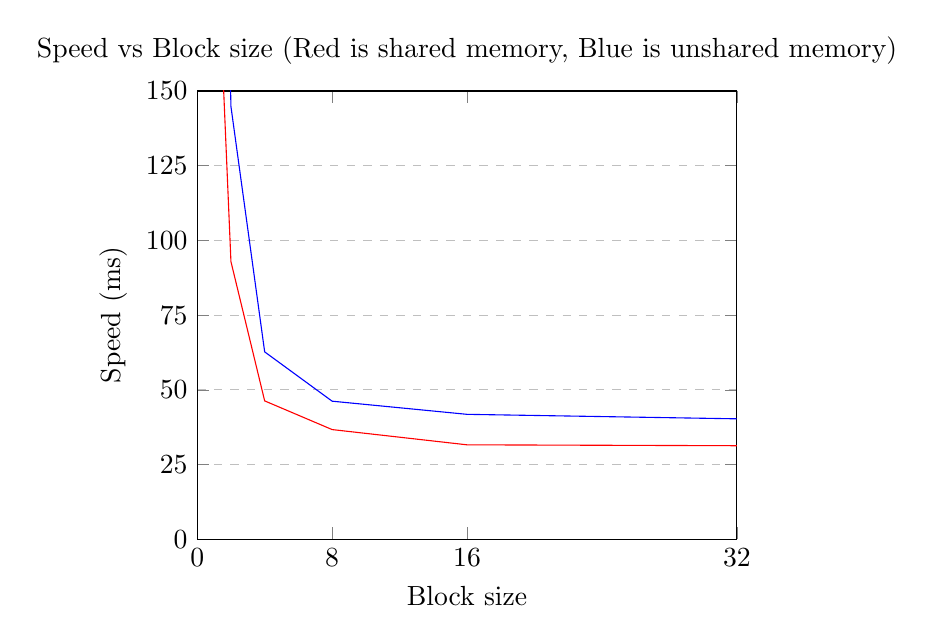
\begin{tikzpicture}

\begin{axis}[
    title={Speed vs Block size (Red is shared memory, Blue is unshared memory)},
    xlabel={Block size},
    ylabel={Speed (ms) },
    xmin=0, xmax=32,
    ymin=0, ymax=150,
    xtick={0,8,16,32},
    ytick={0,25,50,75,100,125,150},
    legend pos=north west,
    ymajorgrids=true,
    grid style=dashed,
]
 
\addplot[
    color=blue,
    ]
    coordinates {
    (1,405.7)(2,144.8)(4,62.7)(8,46.2)(16,41.8)(32,40.3)
    };
\addplot[
    color=red,
    ]
    coordinates {
    (1,225.5)(2,92.9)(4,46.3)(8,36.7)(16,31.6)(32,31.3)
    };
 
\end{axis}
\end{tikzpicture}
%%% End document
\end{document}
